\section{Preliminaries}\label{section:preliminaries}

\subsection{Definitions And Terminology}
%A graph is a 2-tuple consisting of a vertex set and an edge set. The visualization, however, has to be drawn in some kind of way. Investigating the drawing of a graph needs to include several constraints, for example, \emph{how} we want the drawing and \emph{where} we want to draw on. These constraints can be described mathematically.\\
A \emph{graph} $G=(V,E)$ is a tuple consisting of two sets - the set of vertices $V=V(G)$ and the set of edges $E=E(G)$. An \emph{edge} $e = (v,w), v,w \in V$ is a tuple and describes a connectivity relation between two vertices.
% subgraph
If $V'\subseteq V, E'\subseteq E$, then $G' = (V',E')$ is a \emph{subgraph} of $G$.
% degree
The \emph{degree} of a vertex states the amount of edges incident to the vertex.\\
% path
A \emph{path} of length $k$ from a vertex $v_1$ to $v_{k+1}$ is a sequence of vertices $(v_1,...,v_{k+1})$ such that $(v_i,v_{i+1})$ is an edge in $G$.  A path is \emph{simple} if all the vertices in the sequence are distinct. A \emph{cycle} is a path where $v_1 = v_{k+1}$ and has at least one edge. A graph with no cycles is called \emph{acyclic} \cite[P. 1170]{DBLP:cormen_intro_to_algorithms}.\\
% Undirected
Unless otherwise mentioned, the graphs are \emph{undirected}, meaning that the edge $(u,v)$ is identical to the edge $(v,u)$.
% connected 
An undirected graph is \emph{connected} if every vertex is reachable from all the other vertices \cite[P. 1170]{DBLP:cormen_intro_to_algorithms}.
% biconnected
A graph is \emph{biconnected} if the removal of any vertex still leaves the graph connected \cite[P. 224]{Duncan_planar_polyline_drawings}.\\
% simple / multigraph
A graph is \emph{simple} if it does contain neighter multiple edges nor self loops. On the other hand, if a graph contains multiple edges or self loops, it is called a \emph{multigraph} \cite[P. 1172]{DBLP:cormen_intro_to_algorithms}. Unless otherwise mentioned, a graph is presumed to be simple.\\
% Planarity
The \emph{depth-first search, DFS} in short, is a strategy to explore edges out of the most recently discovered vertex $v$ that still has unexplored edges leaving it. Once of all $v$'s edges have been explored, the DFS backtracks in order to explore edges leaving the vertex from which $v$ was discovered. The DFS terminates when all the reachable vertices from the original source vertex were discovered \cite[P.603]{DBLP:cormen_intro_to_algorithms}.

% Graph Drawings

\subsection{Graph Drawing Models And Representations}
% Grid
An $h \times w$ \emph{grid} is a graph consisting of $h$ rows and $w$ columns of vertices. The vertex in the $i$-th row and $j$-th column is denoted as $(i,j)$ and is called a \emph{grid point}. All vertices in a grid have exactly four neighbours, except for the boundary vertices \cite[P. 760]{DBLP:cormen_intro_to_algorithms}. One \emph{unit length} values the distance between two adjacent vertices on the grid and is denoted as \UL.
% Drawing
A \emph{drawing} $\Gamma$ of a graph $G$ is a function, where each vertex is mapped on a unique point $\Gamma(v)$ in the plane and each edge is mapped on an open Jordan curve $\Gamma(e)$ ending in its vertices \cite[P. 225]{Duncan_planar_polyline_drawings}. In this context, a graph will be drawn on an underlying grid.\\
A drawing is called \emph{planar} if no two distinct edges intersect. 
A graph is \emph{planar} if it admits a planar drawing\cite[Page 100]{DBLP:cormen_intro_to_algorithms}.
% Face
A drawing partitions the plane into topologically connected regions \cite[P. 7]{battista_1999}. A \emph{face} is a maximal open region of the plane bounded by edges. The \emph{outer face} is the unbounded face. A bounded face is called \emph{inner face} \cite[S. 86]{Diestel_GraphTheory}.\\
% Dual graph
A multigraph $G^*$ is the \emph{dual graph of $G$} if and only if there exists a bijective function between $G^*$ and $G$ such that:
\begin{enumerate}
	\item Every face $f$ in $G$ corresponds to a vertex $v_f$ in $G^*$
	\item For every edge $e$ of $G$, the corresponding vertices of the faces in $G^*$ incident to $e$ get an edge 
	\item If $e$ is incident to only one face, a loop is attached to the corresponding vertex in $G^*$
\end{enumerate}\cite[P. 103]{Diestel_GraphTheory}
The \emph{weak dual graph} of $G$ is the dual graph of $G$ without considering the outer face.\\

% Embedding
An \emph{embedding} of $G$ is the collection of counter-clockwise circular orderings of edges around each vertex of $V$, denoted as a sequence of edges.\\
% Straight-line drawing
In a \emph{straight-line drawing}, verticees are points on the grid and edges are straight-line segments.\\
% Polyline drawing
In a \emph{polyline drawing}, vertices are points on the grid, edges are sequences of contiguous straight-line segments. The transition point between two edge segments with different slopes is called a \emph{bend}. Like vertices, bends are placed on points on the underlying grid.\\
% Box
A \emph{box} is an axis-parallel rectangle, overlapping vertical and horizontal grid lines. The \emph{width} of a box is one unit smaller than the number of vertical grid lines that are overlapped by it. The \emph{height} of a box is one unit smaller than the number of horizontal grid lines that are overlapped by it.
% Box drawing
In an \emph{orthogonal box drawing}, vertices are axis-aligned boxes (possibly degenerated to a line segment or a point), edges are sequences of contiguous horizontal or vertical line segments. \cite[P. 144ff]{Biedl_SP}\\
% Layering
A \emph{layering} is a mapping $L: V \to \mathbb{N}$ and determines the horizontal grid line placement of a vertex. A layering is \emph{valid}, if $|L(u) - L(v)| \geq 1$ for any edge $(u,v)$ \cite[P. 4]{Ruegg_Layering}.\\
% Area
A drawing whose minimum enclosing box has width $w$ and height $h$ is called a $w\times h$-drawing and inherits area $w\cdot h$ \cite[P. 145]{Biedl_SP}.\\
% Euclidian distance
The \emph{euclidian distance} between two grid points $(x_1,y_1)$ and $(x_2,y_2)$ is defined as $\sqrt{(x_2-x_1)^2 + (y_2-y_1)^2}$.
% Edge length
The \emph{length of a line segment} is defined as the euclidian distance between the end points. The \emph{length of a polyline} is defined as the sum of the individual line segment lengths.

\subsection{The Relationship Between Drawing Models}

Box drawings, straight-line and polyline drawings are the drawings of interest in this thesis. They stand in relation to each other in the following way:\\
A straight-line drawing is a polyline drawing with no bends by definition. Every sequence of line segments is of length 1.\\
A box drawing can be transferred to a polyline drawing with asymptotically the same area consumption. For this to happen, add empty grid lines until every segment of every edge has length at least 2. This will at most double the width and height. For any vertex, replace the box by an arbitrary grid point inside the box and reroute the incident edges to that vertex locally. Every box introduces a bend per edge, resulting in a polyline drawing with two bends and the asymptotically same area bound.
\cite[P. 145]{Biedl_SP}

\begin{figure}[H]
	\centering
	\begin{subfigure}{0.7\textwidth}
		\centering
		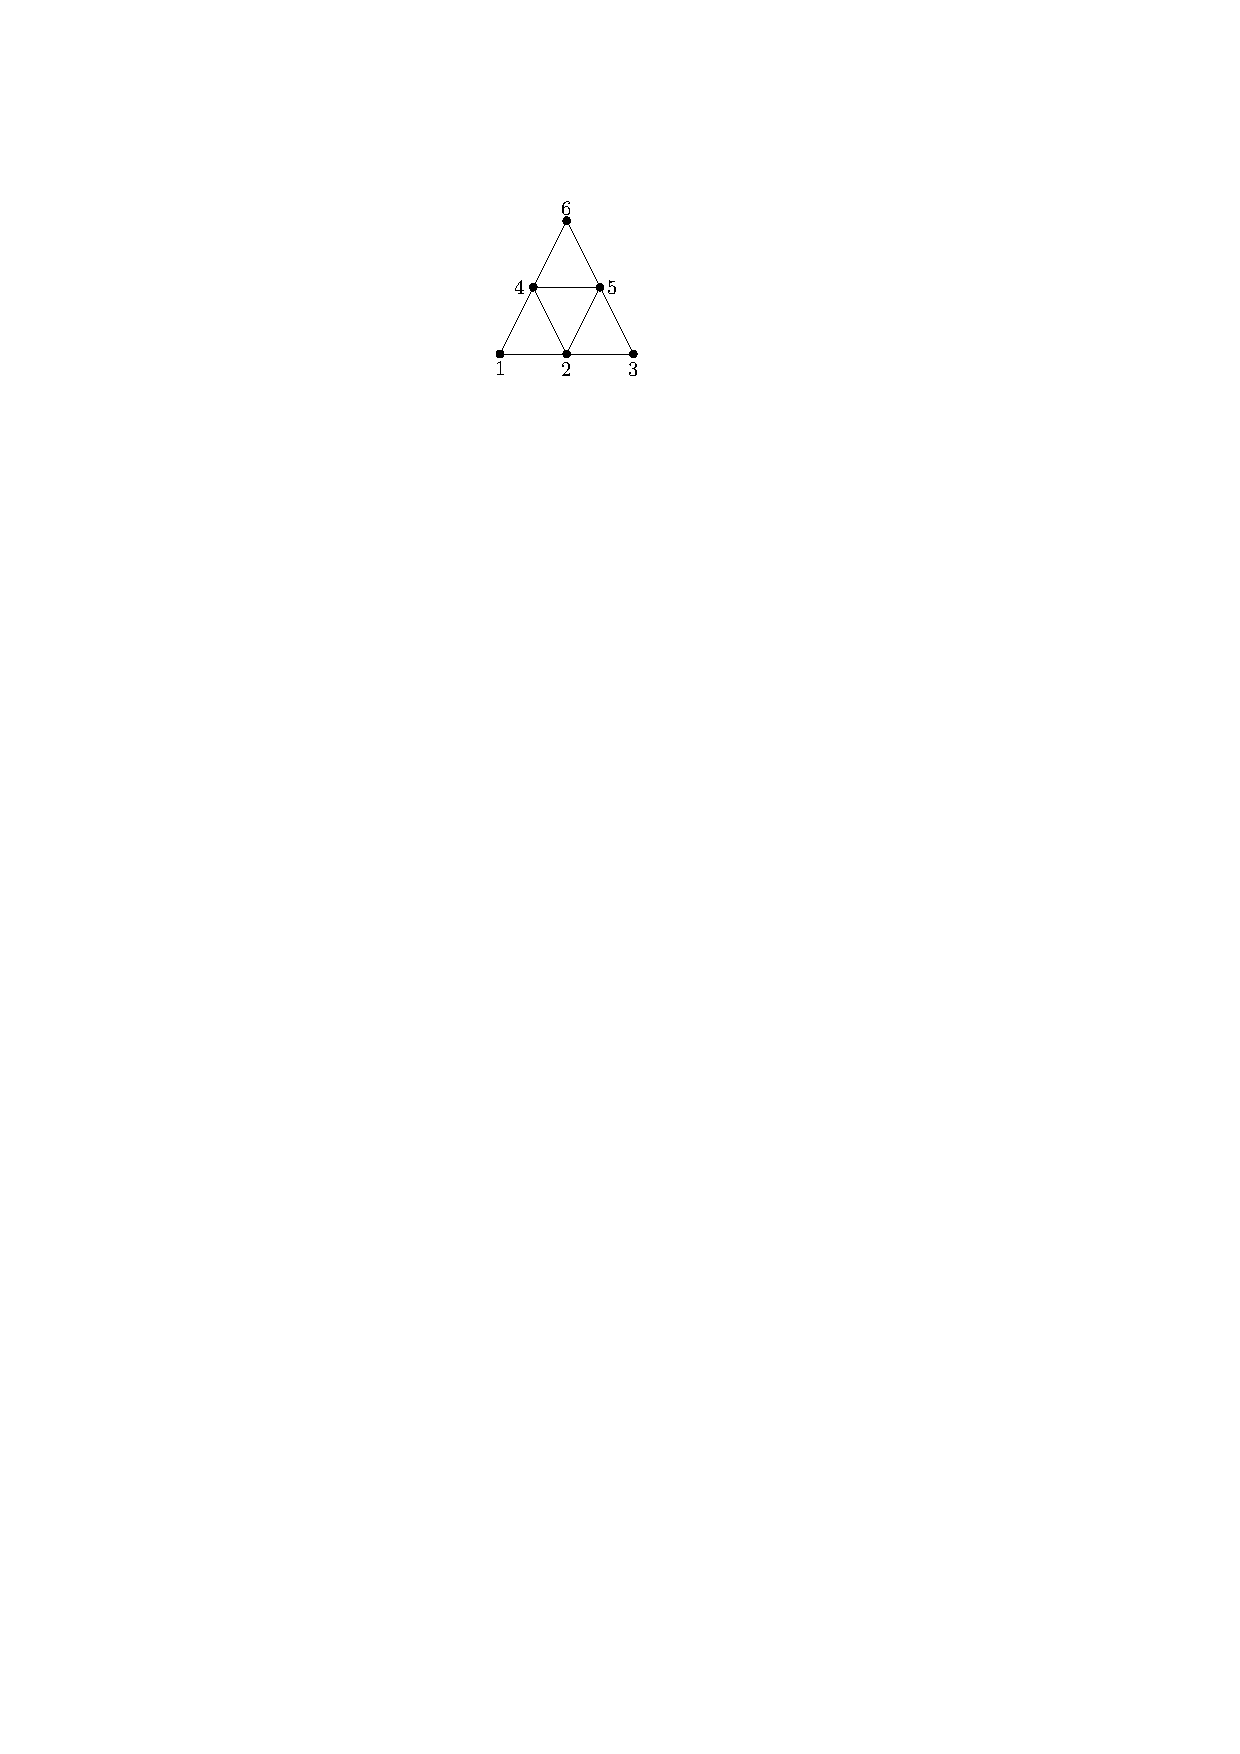
\includegraphics[page=1,width=0.5\linewidth]{graphics/preliminaries_drawing_models.pdf}
		\caption{}\label{im:drawing_models_a}
	\end{subfigure}
\begin{subfigure}{0.4\textwidth}
	\centering
	\includegraphics[page=2,width=\linewidth]{graphics/preliminaries_drawing_models.pdf}
	\caption{}\label{im:drawing_models_b}
\end{subfigure}
\begin{subfigure}{0.4\textwidth}
	\centering
	\includegraphics[page=3,width=\linewidth]{graphics/preliminaries_drawing_models.pdf}
	\caption{}\label{im:drawing_models_c}
\end{subfigure}
	\caption{\ref{im:drawing_models_a} is a straight-line drawing of a maximal outerplanar graph $G$, \ref{im:drawing_models_b} is a box drawing of $G$ and \ref{im:drawing_models_c} is a polyline drawing derived from \ref{im:drawing_models_b}}\label{im:drawing_models}
\end{figure}

\subsection{Graph Classes}
\subsubsection{Tree}
A graph $T$ is called \emph{tree} if and only if it is connected, acyclic and undirected \cite[P. 1172]{DBLP:cormen_intro_to_algorithms}.\\
% rooted
A tree is \emph{rooted} if one of its vertices is distinguished from the other ones, called the \emph{root}. Unless otherwise mentioned, it is assumed that every tree is rooted at the root vertex $r$. 

% path ancestor parent sibling
When considering a path $(r,v_1,...,v_k)$ from $r$ to any other vertex $v_k$, then, the following holds:
\begin{enumerate}
	\item Besides $w$, every vertex of this path is an \emph{ancestor} of $w$
	\item For an edge $(v_i,v_{i+1})$, $v_i$ is called the \emph{parent} of $v_{i+1}$, and $v_{i+1}$ is a child of $v_i$.
	\item The \emph{height} of the root $r$ is set to 0. For a vertex $v$ of $T$ it holds that its height is larger by one unit than its parent.
\end{enumerate}
% leaves, internal nodes
A vertex with no children is called a \emph{leaf}. Any vertex which is not a leaf is called an \emph{internal node}.
% level
A \emph{level} of $T$ consists of all vertices of the same height.
% height
The \emph{height} of $T$ is equal to the largest height of any vertex of $T$. \cite[P. 1176ff]{DBLP:cormen_intro_to_algorithms}
\subsubsection{$k$-ary Tree}
% complete k-ary tree
A \emph{$k$-ary tree} is a rooted tree in which for every vertex has at most $k$ children.
A \emph{complete $k$-ary tree} is a $k$-ary tree in which all leaves have the same height and all internal nodes have $k$ children.
\subsubsection{Outerplanar Graphs, Series Parallel Graphs and 2-Trees}
% outerplanar graph
An \emph{outerplanar graph} is a planar graph that can be drawn without crossing in a way so that all vertices are on the outer face. A \emph{maximal outerplanar graph} is an outerplanar graph to which it is not possible to add an edge without destroying the simplicity, planarity or outerplanarity property. 
% series parallel graph
A \emph{2-terminal series-parallel graph} with terminals $s,t$ is a recursively defined graph with one of the following three rules:
\begin{enumerate}
	\item An edge $(s,t)$ is a 2-terminal series-parallel graph
	\item If $G_i, i = 1,2$, is a 2-terminal series-parallel graph with terminals $s_i,t_i$, then in the serial composition $t_1$ is identified with $s_2$ to obtain a 2-terminal series-parallel graph with $s_1,t_2$ as terminals
	\item If $G_i, i=1,...,k$, is a 2-terminal series-parallel graph with terminals $s_i,t_i$, then in a parallel composition we identify all $s_i$ into one terminal $s$ and all $t_i$ into the other terminal $t$ and the result is a 2-terminal series-parallel graph with terminals $s,t$.
\end{enumerate}
A \emph{series-parallel graph}, \emph{SP-graph} in short, is a graph for which every biconnected component is a 2-terminal series-parallel graph. A SP-graph is \emph{maximal} if no edge can be further added while maintaining a SP-graph. \cite[P. 143ff]{Biedl_SP}\\
% 2-tree
A \emph{$k$-tree} is a recursively defined graph with at least $k+1$ vertices. If $n = k+1$, then the $k$-tree is the complete graph $K_{k+1}$. If $n>{k+1}$, start with a $K_{k+1}$ and every vertex added is adjacent to exactly $k$ adjacent neighbours. The class of \emph{2-trees} correspond to the class of maximal SP-graphs \cite[Page 2]{straight-line_2-trees}.
\subsection{Tools}
% SPQR Tree
\subsubsection{$SPQR$-Tree}
A \emph{cut vertex} in a graph $G$ is a vertex whose removal disconnects $G$. A \emph{separation pair} in $G$ is a pair of vertices whose removal disconnects $G$. A \emph{biconnected component} of $G$ is a maximal (in terms of vertices and edges) biconnected subgraph of $G$. If $G$ contains vertices $s,t$, then $G$ is \emph{$st$-biconnectable} if $G \cup \{s,t\}$ is biconnected. A \emph{split pair} of $G$ is either a separation pair or a pair of adjacent vertices of $G$. A \emph{maximal split component} of $G$ in regard to a split pair $\{u,v\}$ is either an edge $(u,v)$ or a maximal subgraph $G'$ of $G$ such that $G'$ contains $u$ and $v$ and $\{u,v\}$ is not a split pair of $G'$. A vertex $w$ aside from $u$ and $v$ belongs to exactly one maximal split component. A \emph{split component} of $\{u,v\}$ is defined as the union of any number of maximal split components of $\{u,v\}$. A split pair $\{u,v\}$ is \emph{maximal}, if there is no split pair $\{w,z\}$ in $G$ such that $\{u,v\}$ is contained in a split component of $\{w,z\}$.\\
The \emph{SPQR-Tree} $\mathcal{T}$ of $G$ is a recursively defined composition of $G$ with respect to its split pairs. $\mathcal{T}$ is a rooted tree with four types of nodes: $S,P,Q$ and $R$. Any node $\mu$ of $\mathcal{T}$ is related to a planar $uv$-biconnectible multigraph, the so-called \emph{skeleton} of $\mu$, denoted as $sk(\mu)$. $\mathcal{T}$ is recursively defined - Let $(s,t)$ be an edge of $G$, called the \emph{reference edge}. $\mathcal{T}$ is initialized with a $Q$ node $\phi$ as root, representing the edge $(s,t)$. The skeleton of $\phi$ consists of two parallel edges $(s,t)$. One is a \emph{real }edge, one is a \emph{virtual }edge.\\
After the initialization of $\mathcal{T}$ with an arbitrary reference edge, consider a node $\psi$ of $\mathcal{T}$, $G_\psi=\left(V(G),E(G)\setminus\left\{(s,t)\right\}\right)$ and a pair of vertices $\{u,v\}$ of $G_\psi$, called the \emph{poles} of $\psi$.

\begin{description}
	\item[Trivial case] If $G_\psi$ consists of a single edge $(u,v)$, then $\psi$ is a $Q$-node. In this thesis, this case will be denoted as $Q(u,v)$.
	\item[Series case] If $G_\psi$ is not a single edge and not biconnected, then $\psi$ is a $S$-node with at least one cut vertex $c$ between the path between $u$ and $v$. In this thesis, this case will be denoted as $S(u,c,v)$.
	\item[Parallel case] If $G_\psi$ is not a single edge, but biconnected with $\{u,v\}$ as a split pair of $G_\psi$, then $\psi$ is a $P$-node. In this thesis, this case will be denoted as $P(u,v)$.
	\item[Rigid case] If $G_\psi$ is not a single edge, biconnected with $\{u,v\}$ not being a split pair of $G_\psi$, then $\psi$ is a $R$-node. Due to the properties of the graph classes considered in this thesis, this case will not be covered in application and is not of further interest. 
\end{description}
\cite[P. 7-8]{SPQR-Tree}
% Tree decomposition / treewidth 
\subsubsection{Tree decomposition}
Let $G$ be a graph, $T$ a tree, and let $\mathcal{W} = \left(W_t\right)_{t\in T}$ be a family of vertex sets $W_t \subseteq V_G$ indexed by the vertices $t$ of $W$. The pair $(T,W)$ is called a \emph{tree decomposition} of $G$ if it satisfies the following three conditions:
\begin{enumerate}
	\item $V_G = \bigcup_{t\in T}W_t$
	\item For every edge $e\in E_G$ there exists a $t\in T$ such that both ends of $e$ lie in $W_t$
	\item For all $v\in V$, there exists a connected subtree $T'$ in $T$ such that $v \in W_{t'}, t' \in V_{T'}$
\end{enumerate}
\cite[P. 319]{Diestel_GraphTheory}
\\
The \emph{width} of a tree decomposition is defined as 
\begin{align}
	tw((T,W)) = \max\{ |W_t|,t\in V_T \} -1
\end{align}
The \emph{treewidth} of a graph is the least width of any tree decomposition of $G$ \cite[P. 321]{Diestel_GraphTheory}. A graph with a treewidth bound by $k$ is a $k$-tree \cite[P. 5]{k-tree_bounded-treewidth}.
